% Configurazione della pagina
\documentclass[
  12pt,
  a4paper,
  headings=optiontoheadandtoc
]{scrreprt}
\setlength{\parskip}{\baselineskip}
%\pagenumbering{gobble}

% Dichiarazione dei pacchetti utilizzati
\usepackage{ragged2e}
\usepackage{tabularx}
\usepackage{graphicx}

% Metadati per il titolo
\author{Ghellere Nicolò, Milli Manuel, Sacchetto Riccardo}
\date{15 febbraio 2023}
\title{Dispositivo di gestione di un parcheggio}
\subtitle{Elaborato SIS - Relazione}

% Cartella delle immagini
\graphicspath{ {./img/} }


% ===== Inizio del documento =====
\begin{document}

% Creazione del titolo
\maketitle

% Configurazione e creazione della ToC
\renewcommand*\contentsname{Indice}
\tableofcontents
\newpage

\chapter[nonumber=true]{Architettura del dispositivo}

Lo scopo del dispositivo descritto in questa relazione e realizzato sotto forma di circuito digitale in formato BLIF per SIS è quello di gestire un parcheggio con ingresso e uscita automatizzati, ricevendo in input l'azione dell'utente (ingresso o uscita) e il settore d'interesse (A, B o C) e aprendo la sbarra d'ingresso o uscita a patto che il settore selezionato non sia, rispettivamente, pieno o vuoto.

L'input è costituito da cinque bit: due per l'azione (ingresso=01, uscita=10) e tre per il settore (A=100, B=010, C=001); l'output è invece costituito da sei bit: uno che rappresenta la scelta di un settore non valido, due che comunicano quando aprire la sbarra d'ingresso (10) o quella d'uscita (01) e tre che segnalano i settori pieni (il primo per A, il secondo per B e il terzo per C).

I due componenti logici del dispositivo sono la FSM con i cinque stati che rappresentano le fasi del ciclo di funzionamento e il datapath che si occupa di memorizzare, aggiornare e analizzare la quantità di veicoli nei vari settori, tenendo conto che in A e B ci possono essere fino a un massimo di 31 veicoli e in C un massimo di 24.

\section[nonumber=true]{La FSM}

La FSM che funge da controller per il circuito di controllo del parcheggio presenta cinque stati diversi:

\begin{itemize}
  \item \textbf{OFF}: Rappresenta lo stato d'inattività del dispositivo. Finchè si trova in questo stato il circuito attenderà la sequanza di avvio \textbf{11111} ignorando ogni altro input e ponendo a 0 ogni bit di output
  \item \textbf{READA}: Primo stato di avvio. L'input ricevuto in questo stato verrà interpretato come il numero di veicoli posizionatisi nel settore A durante l'inattività del sistema di controllo
  \item \textbf{READB}: Secondo stato di avvio. L'input ricevuto in questo stato verrà interpretato come il numero di veicoli posizionatisi nel settore B durante l'inattività del sistema di controllo
  \item \textbf{READC}: Terzo stato di avvio. L'input ricevuto in questo stato verrà interpretato come il numero di veicoli posizionatisi nel settore C durante l'inattività del sistema di controllo
  \item \textbf{RDY}: Normale stato di funzionamento. Finchè si trova in questo stato il dispositivo risponderà alle richieste d'ingresso o uscita degli utenti, alzando e abbassando le sbarre e comunicando i settori pieni. Il sistema tornerà nello stato \textbf{OFF} quando riceverà la squenza \textbf{00000}
\end{itemize}

Internamente, al fine di comunicare con il datapath e di controllarne il funzionamento la FSM utilizzerà i seguenti segnali:

\begin{itemize}
  \item \textbf{WA}: Segnala al datapath quando interpretare l'input come numero di posti occupati in A durante la notte. Posto a 1 solo in \textbf{READA}
  \item \textbf{WB}: Segnala al datapath quando interpretare l'input come numero di posti occupati in B durante la notte. Posto a 1 solo in \textbf{READB}
  \item \textbf{WC}: Segnala al datapath quando interpretare l'input come numero di posti occupati in C durante la notte. Posto a 1 solo in \textbf{READC}
  \item \textbf{OPENPARKS}: Segnala quando il dispositivo è pronto a ricevere le query degli utenti aprendo le sbarre in risposta a esse. Posto a 1 da \textbf{RDY}
  \item \textbf{SHOWFULLA}: Segnala al datapath quando mostrare se il settore A è pieno. Posto a 1 da tutti gli stati consecutivi a \textbf{READA}
  \item \textbf{SHOWFULLB}: Segnala al datapath quando mostrare se il settore B è pieno. Posto a 1 da tutti gli stati consecutivi a \textbf{READB}
  \item \textbf{SHOWFULLC}: Segnala al datapath quando mostrare se il settore C è pieno. Posto a 1 da tutti gli stati consecutivi a \textbf{READC}
  \item \textbf{INVSEC}: Mappato al primo bit dell'output generale, segnala quando l'utente ha immesso un settore non valido. Può essere posto a 1 da \textbf{RDY}
\end{itemize}

Per meglio comprendere il funzionamento del controller segue il digramma degli stati della FSM che lo costituisce. I bit di input sono elencati come da specifica mentre quelli di output sono nell'ordine descritto dall'elenco appena riportato:

\Centering
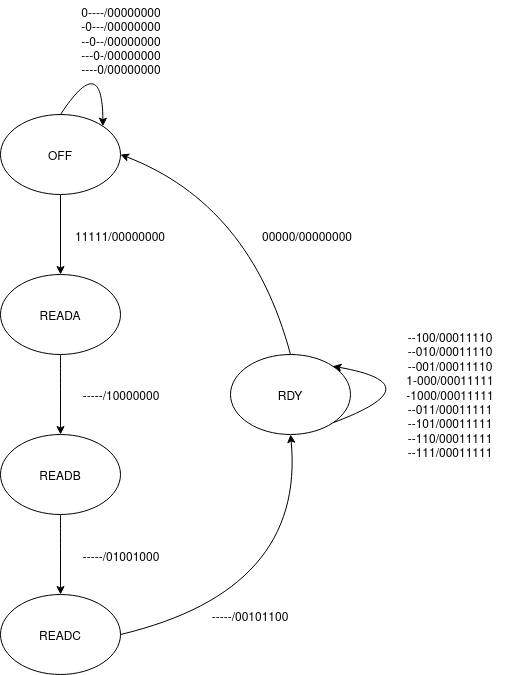
\includegraphics[scale=0.75]{controller}

\RaggedRight

\section[nonumber=true]{Il DataPath}

\Centering
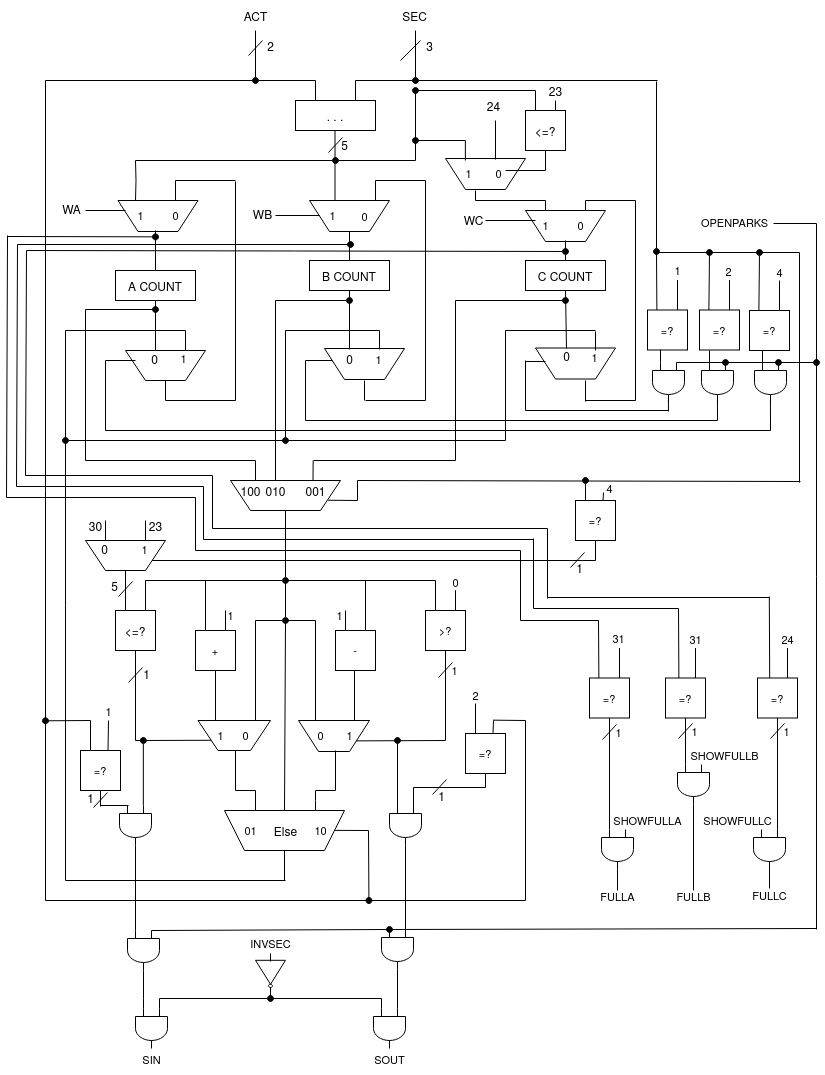
\includegraphics[scale=0.5]{datapath}

\RaggedRight

Come è possibile notare osservando il diagramma riportato, il datapath è composto da due parti principali: la logica di caricamento e di gestione dei registri e la logica di aggiornamento del conteggio d'interesse per la richiesta effettuata dall'utente.

Le due parti sono separate dal one-hot multiplexer a tre ingressi collocato al centro del diagramma, il quale riceve in input tutti e tre i conteggi salvati al ciclo precedente e trasmette alla logica di calcolo solo quello che corrisponde al parcheggio d'interesse dell'utente.

\subsection[nonumber=true]{Gestione dei registri}
\end{document}
